\chapter{Organizational Social Networks}
\section{Application of Social Networks to OSS Research}
In research projects concerning OSS, social networks are a useful tool to build understanding of the overall structure and flow of the distributed collaboration. Madey, Freeh, and Tynan\cite{madey2002open}, for instance, used social networks to perform an empirical study of collaboration on SourceForge projects, finding that the number of developers per project and the number of projects per developer both have power-law distributions. Similarly, by modeling organizational collaborations in ASF projects as a social network, we can answer questions about the high-level scope and structure of organizational involvement in ASF.

For the present study, social networks were employed to find out the centralization level of organizational contributions to ASF, and to pinpoint the organizations which are most central to ASF project development. In addition to computing these values, the social networks were plotted using R, which provided an visual overview of the network structure. Afterwards, some of the most interesting phenomena observed in these network analyses were investigated in more detail, in order to better understand what caused them to appear, and what effects they have on the network.
\section{Building the Network}
Once the contributors' commit counts and employers were known, a social network of organizations was created based on the shared collaborations of their members. This was done in the following steps:
\begin{enumerate}
	\item The \textbf{companyprojectcommitcount} table was joined with itself on column \textbf{project} and the two commit counts of each row were summed into one, creating an edge list for companies, with the summed commit count as the edge weight.
	\item The edge list was imported into R, symmetric edges were removed, and edges connecting the same vertices were merged by summing their commit counts.
	\item Networks were created using R packages \textbf{network} and \textbf{igraph}.
\end{enumerate}
Essentially, there was an undirected edge between organizations A and B when a member of A and a member of B committed to the same project. The edge weight was the sum of the number of commits from A's members and the number of commits from B's members to all projects where they both contributed.

\section{Network Plots}
One challenge in plotting complex networks is that when there are many nodes and edges, it becomes difficult to discern the structure of a network by looking at the plot, especially if it was plotted using a simple algorithm. Since the organizational network had 90 vertices and 622 edges, a more sophisticated plotting approach was necessary. In their 2004 paper\cite{gonzalez2004community}, Gonz{\'a}lez-Barahona, L{\'o}pez, and Robles demonstrated that the Girvan-Newman (GN) algorithm can generate a hierarchical graph layout, which makes it easier to visually identify graph structure. They applied this method to plotting a network of developers of the Apache HTTP Server, the founding project of the ASF, and asserted that the GN algorithm provides ``a step forward at least in the aspect of offering a way to visually identify an affiliation network,'' compared to the classical network analysis algorithms used by previous works. Since the GN algorithm was shown to be effective for highlighting the structure of Apache developer network, it was applied for plotting the ASF organizational network.

An image of the plot is shown in figure \ref{fig:orgCommunities}. This plot was generated using the R package \verb|igraph|, which contains a function named \verb|edge.betweenness.community| that implements the GN algorithm to generate a ``communities'' object. Communities highlight graph structure by grouping vertices into different neighborhoods based on their edges. In the figure, each community is shaded with a different color, and vertices in the same community are colored the same, making it easier to see the relationships between clusters. Edge weights are not reflected in this graph, as the vertices could not be spread out far enough to allow increasing edge thickness without causing disruption.

In looking at the graph, it is immediately apparent that there are identifiable clusters of organizations that are in close collaboration, and there are a few ``linchpin'' organizations which connect these clusters. Although the center cluster is still a bit too cluttered, the easy identifiability of the communities and the vertices connecting them provides further evidence that hierarchical algorithms such as GN are well-suited for the task of exhibiting the structure of complex social networks. A closer analysis of the clusters is provided in section \ref{clustersection}.
\begin{figure}
	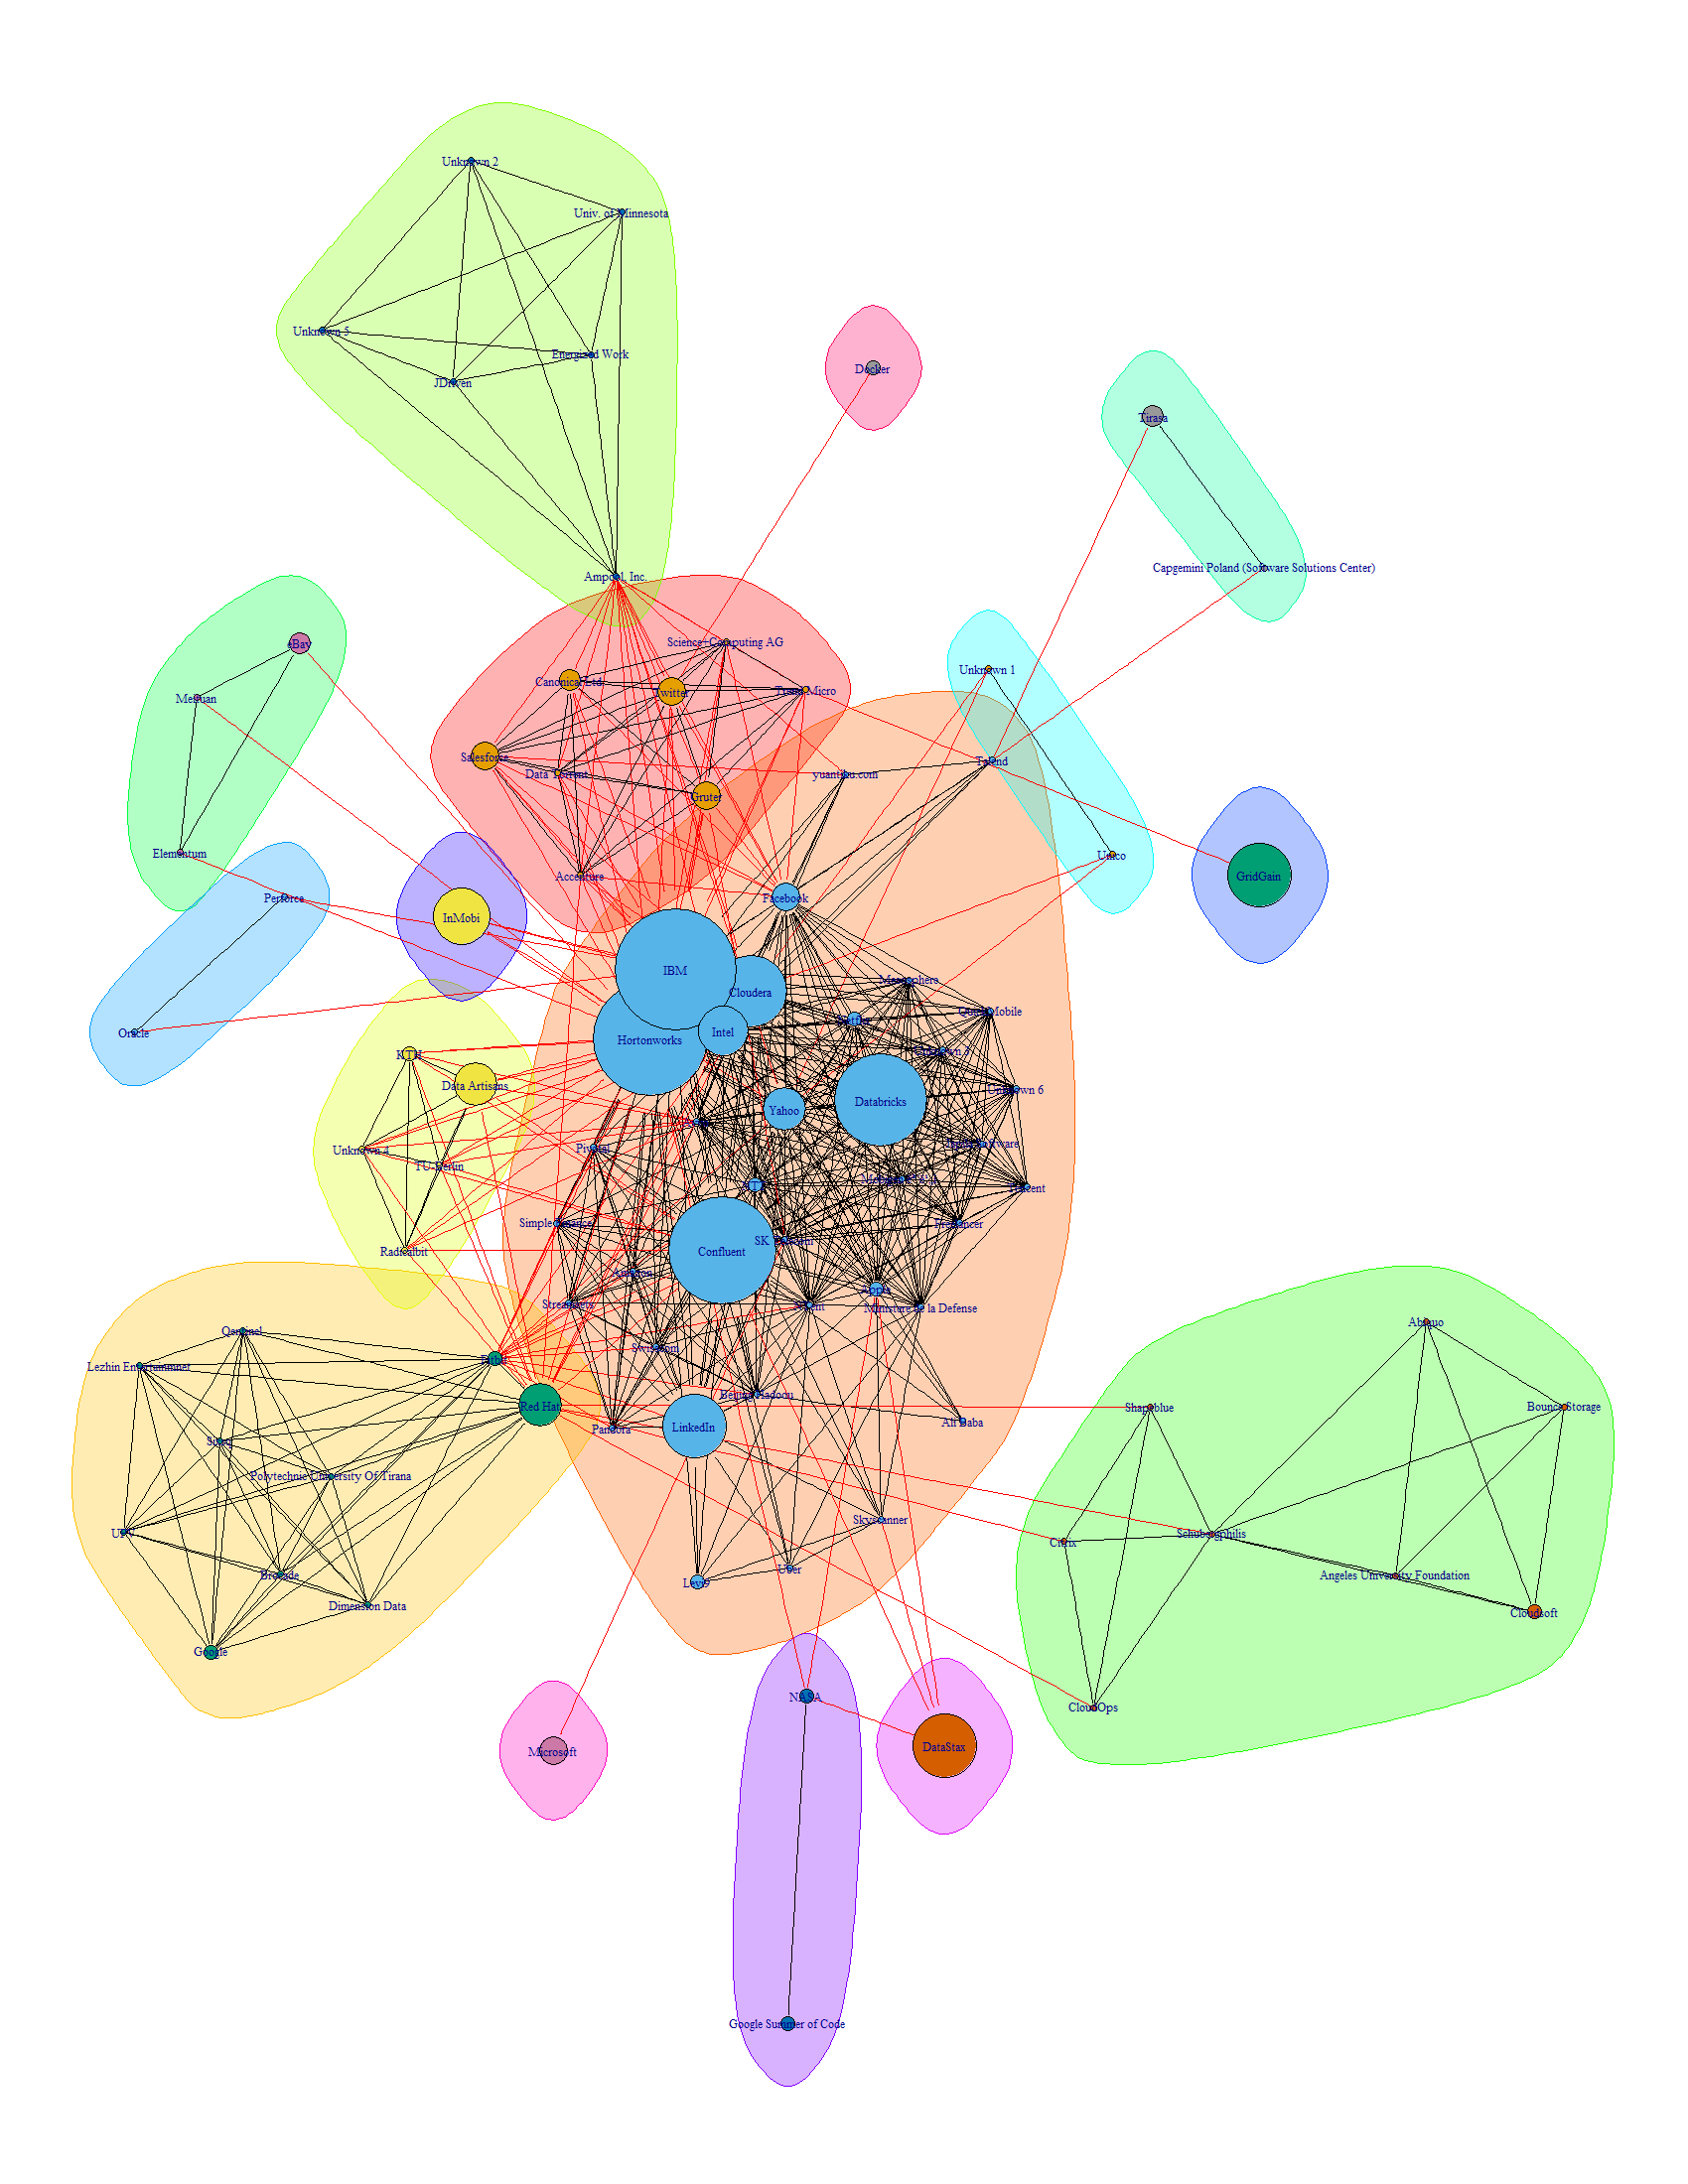
\includegraphics[width=\textwidth]{communities.png}
	\centering
	\caption{The organizational communities}
	\label{fig:orgCommunities}
\end{figure}

\section{Centrality Measures}

\section{Cluster Analysis}\label{clustersection}